\documentclass{beamer}

\usepackage[T2A]{fontenc}
\usepackage[utf8x]{inputenc}
\usepackage[english,bulgarian]{babel}
\usepackage{multirow}

\mode<presentation> {
	\usetheme{Berlin}
}

%\usebackgroundtemplate {
%	\includegraphics[width=370px, height=270px, trim=0 0 0 -80px]{background}
%}

\graphicspath{{../images/}}

\title{Оператори за контрол на изпълнението и потребителски функции}
\subtitle{Статистическа обработка на данни с R}

\author{Пламен Петров и Тодор Балабанов}

\date{22.V.2020}

\institute[ЦО и ИИКТ към БАН] {
	Център за обучение \\
	Институт по информационни и комуникационни технологии \\ 
	Българската академия на науките \\
	\medskip
	\textit{p.petrov@iit.bas.bg todorb@iinf.bas.bg}
}

\addtobeamertemplate{navigation symbols}{}{
	\usebeamerfont{footline}
	\usebeamercolor[fg]{footline}
	\hspace{1em}
	\insertframenumber/\inserttotalframenumber
}

\begin{document}

\begin{frame}
	\titlepage
\end{frame}

\section*{Теми}
\begin{frame}[shrink]
	\frametitle{Съдържание}
	\tableofcontents
\end{frame}

\section{Организация на експериментите}

\begin{frame}
\center \huge{Организация на експериментите}
\end{frame}

\subsection{Скриптови езици}

\begin{frame}
\frametitle{Последователност от инструкции}
\begin{block}{Примерен R скрипт}
rm(list = ls());

sayHello <- sample(c(TRUE,FALSE), 1, TRUE);

if(sayHello == TRUE) \{

	print( $"$Hello!$"$ );
	
\}

print( $"$Bye!$"$ );
\end{block}

\begin{block}{Адрес на скрипта}
https://raw.githubusercontent.com/TodorBalabanov/Statistical-Data-Processing-with-R/master/code/example0001.r
\end{block}
\end{frame}

\begin{frame}
\frametitle{Текстов редактор към продукта R}
\begin{figure}[]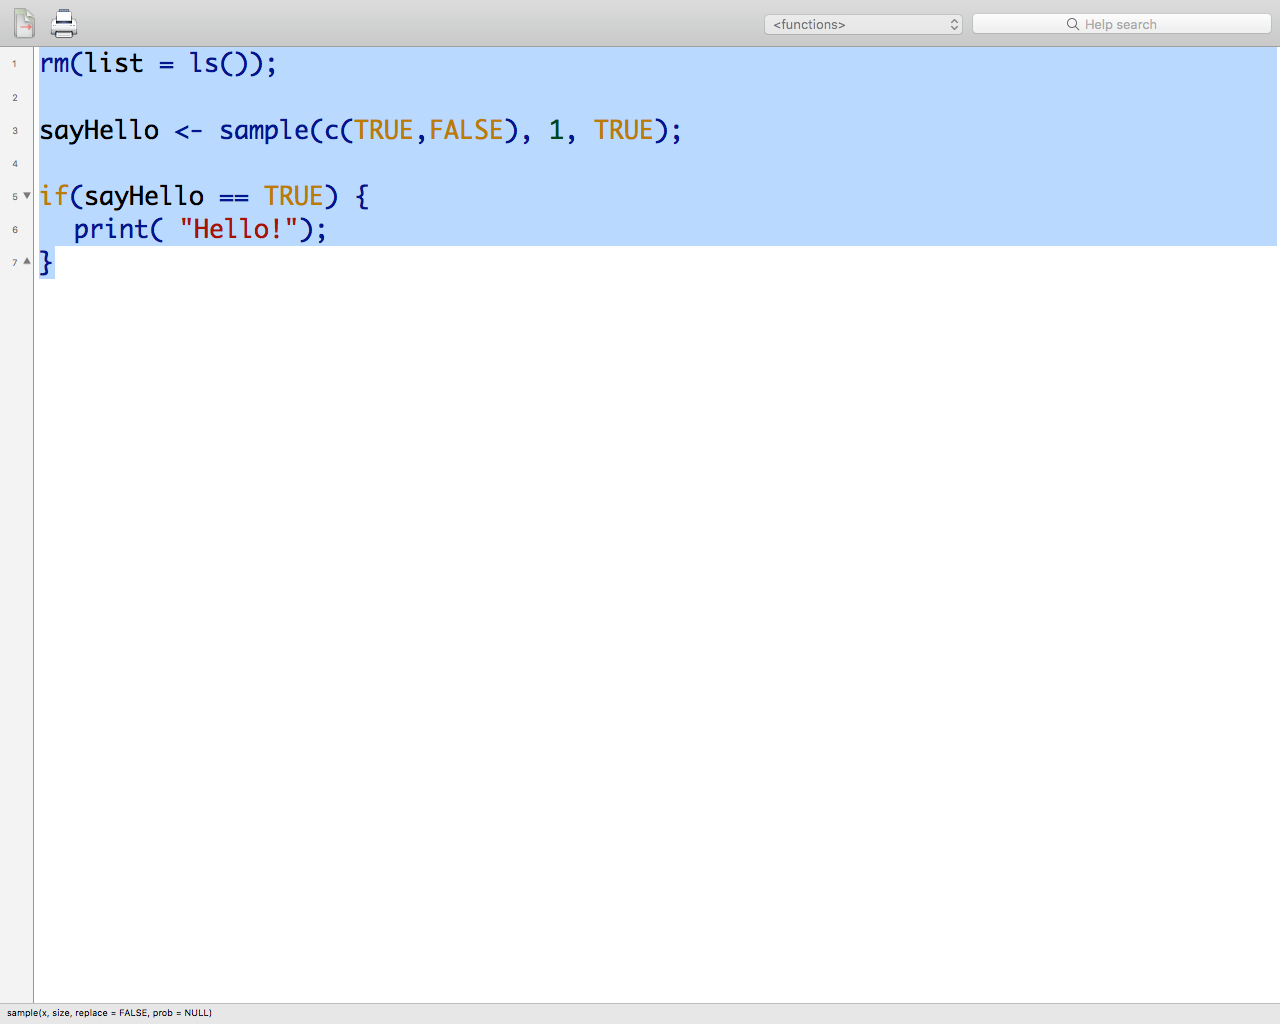
\includegraphics[width=\textwidth,height=0.75\textheight]{pic0025}\end{figure}
\end{frame}

\begin{frame}
\frametitle{Стартиране на R скрипт}
\begin{figure}[]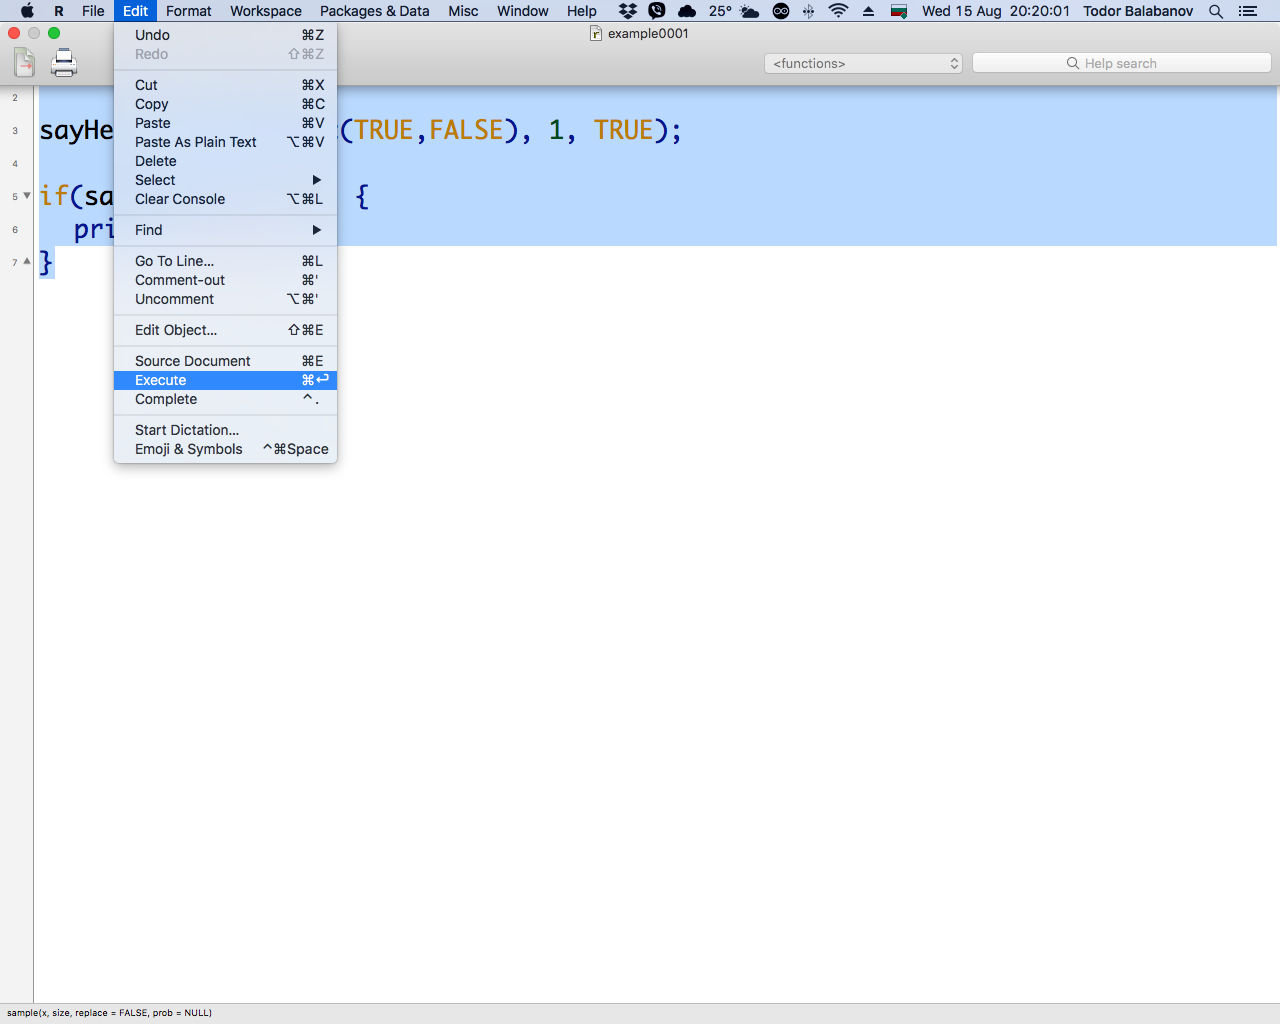
\includegraphics[width=\textwidth,height=0.75\textheight]{pic0026}\end{figure}
\end{frame}

\begin{frame}
\frametitle{Резултат от изпълнението на R скрипт}
\begin{figure}[]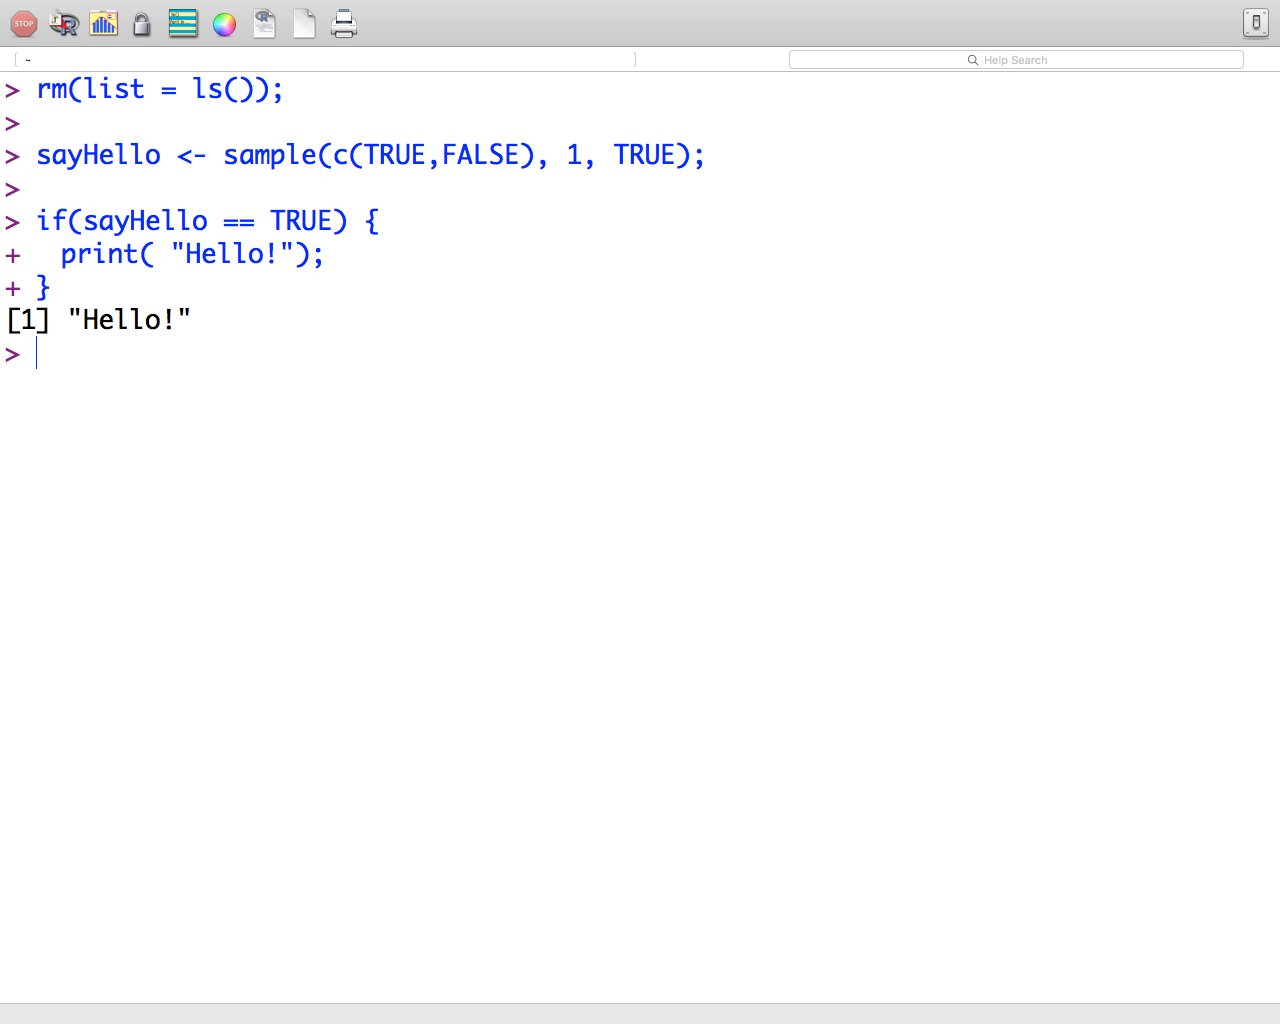
\includegraphics[width=\textwidth,height=0.75\textheight]{pic0027}\end{figure}
\end{frame}

\begin{frame}
\frametitle{Резултат от изпълнението на R скрипт в конзолата на операционната система}
\begin{figure}[]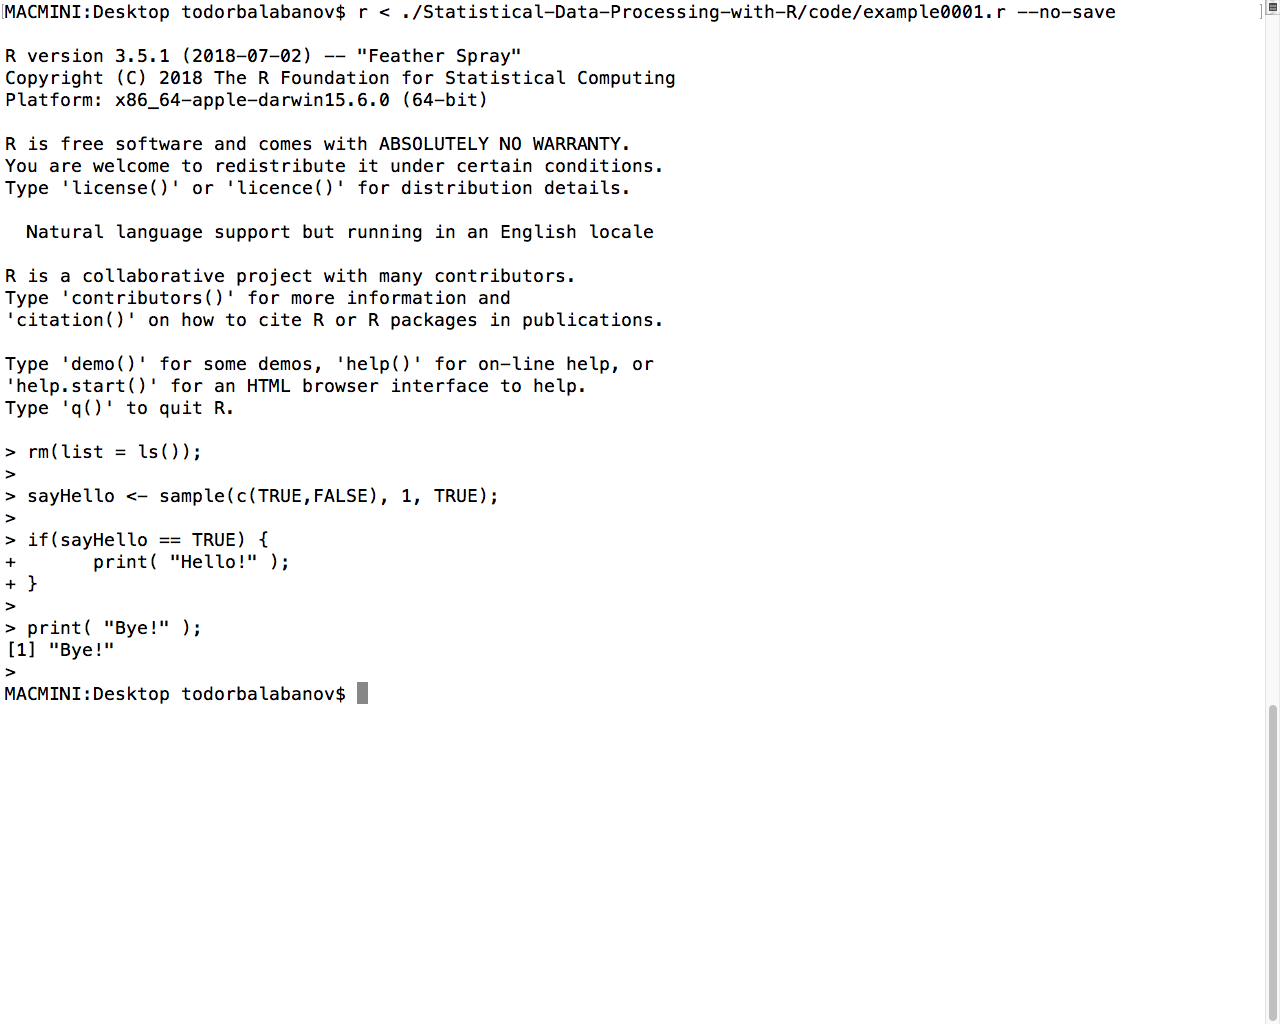
\includegraphics[width=\textwidth,height=0.75\textheight]{pic0028}\end{figure}
\end{frame}

\section{Оператори за преход}

\begin{frame}
\center \huge{Оператори за преход}
\end{frame}

\subsection{Оператор за условен преход}

\subsection{Алтернатива при условен преход}

\subsection{Каскада от условни преходи}

\subsection{Оператор за многовариантен избор}

\section{Оператори за цикъл}

\begin{frame}
\center \huge{Оператори за цикъл}
\end{frame}

\subsection{Цикъл за обхождане}

\subsection{Цикъл с условие за край}

\subsection{Прекъсване на циклите}

\section{Потребителски функции}

\begin{frame}
\center \huge{Потребителски функции}
\end{frame}

\subsection{Аргументи на функция}

\subsection{Аргументи с подразбираща се стойност}

\subsection{Променлив брой аргументи}

\subsection{Върната стойност}

\subsection{Предаване на функция като аргумент}

\section{Заключение}

\begin{frame}
\center \huge{Заключение}
\end{frame}

\subsection{Дискусия}

\begin{frame}
\frametitle{Въпроси и отговори}
\center \huge{Благодаря за вниманието!}
\end{frame}

\end{document}
